\documentclass[tikz, border = 5pt]{standalone}
\usetikzlibrary{quotes,angles}
\usepackage{tkz-euclide}
\usetkzobj{all}
\begin{document}
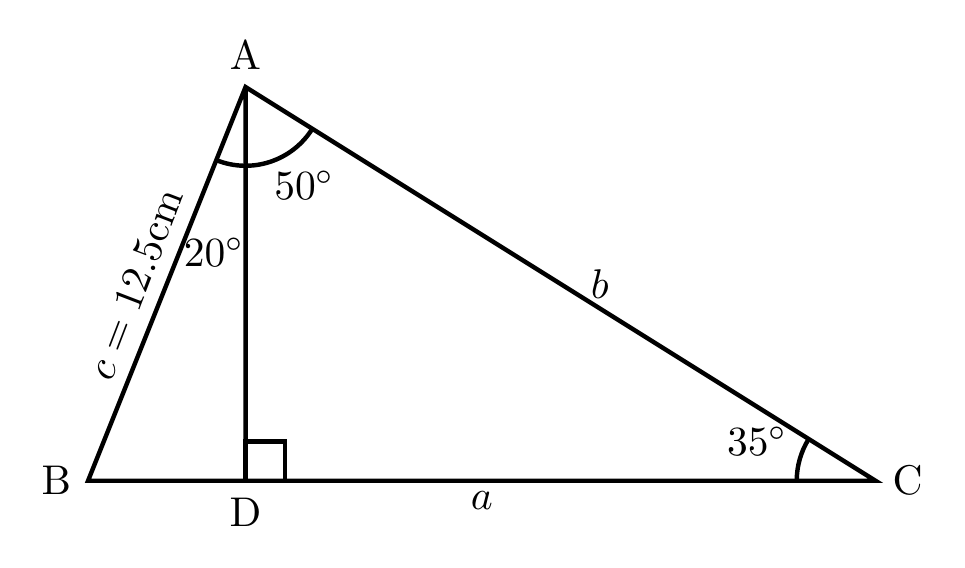
\begin{tikzpicture}
  \draw[ultra thick]
    (0,0) coordinate (b) node[left, scale=1.5] {B}
    -- (10,0) coordinate (c) node[right, scale=1.5] {C}
    -- (2,5) coordinate (a) node[above, scale=1.5] {A}
   -- cycle
   (2,0) coordinate (d) node[below, scale=1.5] {D} -- (2,5)

    pic[draw=black, angle eccentricity=1.3, angle radius=1cm]
    {angle=b--a--c}
    pic[draw=black, angle eccentricity=1.3, angle radius=1cm]
    {angle=a--c--b};
   \tkzMarkRightAngle[ultra thick, draw=black, size=.5](c,d,a);

  \node[scale=1.5] at (5,-.25) {$a$};
  \node[scale=1.5, rotate=69] at (.6,2.5) {$c = 12.5 \mbox{cm}$};
  \node[scale=1.5] at (6.5,2.5) {$b$};
  \node[scale=1.5] at (1.6,2.9) {$20^\circ$};
  \node[scale=1.5] at (2.75,3.75) {$50^\circ$};
  \node[scale=1.5] at (8.5,.5) {$35^\circ$};


\end{tikzpicture}
\end{document}
